\documentclass[prc,amsmath,twocolumn,superscriptaddress]{revtex4}
%\bibliographystyle{prsty}
\usepackage{gensymb}
\usepackage{graphicx,color}
\usepackage{amssymb}
\usepackage{enumerate}
\usepackage{verbatim}
\usepackage{natbib}


\begin{document}

  \newcommand {\nc} {\newcommand}
  \nc {\Sec} [1] {Sec.~\ref{#1}}
  \nc {\IR} [1] {\textcolor{red}{#1}} 

\title{PHY905 Project 4 - Ising Model}


\author{Alaina~Ross}

\date{\today}

%%%%%%%%%%%%%%%%%%%%%%%%%%%%%%%%%%%%%%%%%%%%%%%%%%%%%%%%%%%%%%%%%%%%%%%%%%%%%%%%%%%%%%%%%%%%%%%%%%%%%%%%%%%%%%%%%%%%%%%%%%%%%%%%%%%

\begin{abstract}
 \noindent {\bf Background:} A fairly accurate model of the solar system can be achieved with the use of newtonian mechanics. However, this leads to many coupled differential equations which are difficult to solve analytically.
\\ {\bf Purpose:} The goal of this work is to solve the Ising model in two dimensions to probe the properties of phase transitions in magnetic materials.
\\ {\bf Method:} We use the Metropolis algorithm to generate the possible spin configurations on the lattice and the Grand Canonical ensemble to analyze the statistical physics at play.
\\ {\bf Results:} We find the the Euler method is unstable even in the binary Earth-Sun system, and causes non-conservation of both energy and angular momentum. In contrast, the velocity Verlet method is found to be very stable and enforces conservation of energy and angular momentum.
 \\ {\bf Conclusions:} Our results demonstrate both the importance of an effective differential equation solver, and that the sun (due to its large mass) essentially controls all of the dynamics of the other bodies in the system. 
\end{abstract}


\maketitle

%%%%%%%%%%%%%%%%%%%%%%%%%%%%%%%%%%%%%%%%%%%%%%%%%%%%%%%%%%%%%%%%%%%%%%%%%%%%%%%%%%%%%%%%%%%%%%%%%
\section{introduction}
\label{intro}
While there are many types of magnetism in physics, the strongest and most common type one encounters in everyday life is ferromagnetism, in which a metal, such as iron or cobalt, becomes permanently magnetized when exposed to a magnetic field. This phenomenon is initiated by a quantum mechanical interaction which causes the spins of unpaired electrons to align, acting against the thermodynamic tendency to randomize the spins.

One of the most common ways to analyze magnetism is the Ising model, in which the magnetic material is treated as a lattice of atomic spins which interact with each of their nearest neighbors. In this model, at low temperatures the system exhibits spontaneous magnetization wherein the average magnetization is nonzero. As the temperature increases the system undergoes a second order phase transition at a specific temperature, known as the critical temperature. In a second order phase transition the two phases on either side of the transition are identical and the transition manifests as a discontinuity in the derivative of the energy, which is different from a first order transition (such as evaporation) in which the two different phases coexist at the critical temperature and the transition manifests as a discontinuity of the energy.

In this work, we implement the metropolis algorithm with the ising model in two dimensions in order to study phase transitions of magnetic systems. Calculations of the average energy, heat capacity, average magnetization and the susceptibility are performed and compared to the expected values for a small system. In addition, the behavior of these quantities as a function of temperature is analyzed in order to extract the critical temperature of the phase transition. Finally, the performance of the metropolis algorithm is analyzed. In Sections \ref{theory} and \ref{methods}, the necessary theory and implementation of the algorithms are described. In Section ~\ref{results} the performance and accuracy of the code are analyzed. Finally, in Section \ref{conc} we give a summary and our conclusions.

\section{theory}
\label{theory}
In this work we will use the Canonical ensemble, where the probability of a given state $i$ is given by the Boltzman distribution (with the Boltzman constant set to one):
\begin{equation}
P_i(T) = \frac{e^{-E_i/T}}{Z}
\end{equation}
where Z is the partition function given by the following sum over all possible states:
\begin{equation}
Z=\sum_i e^{-E_i/T}.
\end{equation}
The energy of a particular microstate is given by:
\begin{equation}
E= -J\sum_{\langle kl \rangle} s_ks_l-B\sum_k s_k
\end{equation}
where $J$ is a coupling constant, $B$ is the external magnetic field and $s_{k,l}$ are the spins. In this work, the coupling constant is taken to be one and there is no external magnetic field.

\begin{table}[b]
\centering
\begin{tabular}{|c|c|c|c|}
\hline
Number of spins up & ~Degeneracy ~& ~ $E_i$ ~& ~ $M_i$ ~\\
\hline
4&1&-8&4\\
3&4&0&2\\
2&4&0&0\\
2&2&8&0\\
1&4&0&-2\\
0&1&-8&-4\\
\hline
\end{tabular}
\caption{Energy and magnetization of all possible spin configurations for a 2x2 lattice.}
\label{states}
\end{table}

For a simple 2x2 lattice the possible states are given in Table~\ref{states} and the partition function is given by:
\begin{equation}
Z = 2e^{8/T}+2e^{-8/T}+12.
\end{equation}
Similarly the average energy and average squared energy are given by:
\begin{gather}
\langle E\rangle= \sum_i E_i e^{-E_i/T} = -16e^{8/T}+16e^{-8/T}\\
\langle E^2\rangle= \sum_i E^2_i e^{-E_i/T} = 128e^{8/T}+128e^{-8/T}.
\end{gather}
From these quantities we can calculate the energy variance, which is related to the heat capacity by:
\begin{gather}
C_V = \frac{1}{T^2} \left(\langle E^2\rangle-\langle E\rangle^2\right) \notag \\
= \frac{1}{T^2} \left(128e^{-8/T}-128e^{8/T}+512\right)
\end{gather}

Similarly, one can calculate the average magnetization, average square magnetization, and the magnetic susceptibility as:
\begin{gather}
\langle |M|\rangle= \sum_i |M_i| e^{-E_i/T} = 8e^{8/T}+8\\
\langle M^2\rangle= \sum_i M^2_i e^{-E_i/T} = 32e^{8/T}+32 \\
\chi = \frac{1}{T} \left(\langle M^2\rangle-\langle |M|\rangle^2\right)= \frac{1}{T} \left(-96e^{8/T}-32\right).
\end{gather}
%These analytic values can then be compared to the calculated ones for a 2x2 lattice to ensure that the calculations are being performed correctly.

In the Canonical ensemble the important potential is the Helmholtz free energy, which is given by:
\begin{equation}
F = -TlnZ.
\end{equation}
The average energy and heat capacity can then also be related to the first derivative of the Hemlholtz energy as:
******THESE EQNS NEED TO BE FIXED LATER***
\begin{gather}
\langle E \rangle = T^2\left( \frac{\partial lnZ}{\partial T}\right)_{V,N} \\
C_{V}=-\frac{1}{T^2}\frac{\partial^2 (TlnZ)}{\partial T^2}
\end{gather}

As discussed in Section~\ref{intro}, the phase transition will manifest as a discontinuity in the derivative of the energy (thus the heat capacity). However, near the critical temperature ($T_C$), the dependance of several physical quantities on temperature can be expressed using the following power laws:
\begin{gather}
\langle M(T) \rangle \sim (T-T_C)^\beta \\
C_V(T)\sim |T_C -T|^{-\alpha} \\
\chi(T) \sim |T_C-T|^{-\gamma}
\end{gather}
where the exponents are given by $\beta$ = 1/8, $\alpha$ = 0, and $~\gamma$ = $-7/4$.
\section{methods}
\label{methods}
For an NxN lattice, the number of spin configurations is given by $2^{N^2}$. From Equations 5-10, we see that in order to calculate the various physical quantities of interest, we must sum over all possible microstates, however this is not trivial to perform computationally. To solve this problem we use the Metropolis algorithm~\cite{met} to generate a new configuration from the previous one. 

In the Metropolis algorithm, we pick a random spin and determine the change in energy of the system when the spin is flipped. If that energy is less than the previous energy we accept the transition, if not then we calculate the value $w=e^{\Delta E/T}$ and generate a random number, $r$. If the random number is less than $w$, then the move is also accepted. This constitutes one Monte Carlo cycle, and is repeated until some maximum number of cycles has been achieved  that presumably ensures all configurations have been tested.

As the lattice in our calculations is of dimension $N^2$ rather than infinite, there will be edge spins which have fewer neighbors than the rest. To get around this we will use periodic boundary condititons, where for example the top left spin's "top" neighbor is the bottom left spin etc.

In addition, the lack of an infinite lattice means the behavior near the critical temperature will be modified from Equations 13-15, namely:
\begin{gather}
\langle M(T) \rangle \sim N^{-\beta/\nu} \\
C_V(T)\sim N^{\alpha/\nu} \\
\chi(T) \sim N^{\gamma/\nu}
\end{gather}
where $\nu$ is defined by the relationship between the infinite critical temperature and the calculated critical temperature:
\begin{equation}
T_C(N)-T_C(N=\infty) \sim aN^{-1/\nu}
\end{equation}
where a is a constant.

\section{results}
\label{results}
We first aim to ensure the algorithm is working as expected by comparing the output for a 2x2 lattice to Equations 5-10. The number of Monte Carlo (MC) cycles needed for 0.1\% agreement is given in Table~\ref{cycles}.

\begin{table}[b]
\centering
\begin{tabular}{|c|c|c|}
\hline
Quantity& Error (\%) & MC cycles\\
\hline
$\langle E\rangle$&0.004 &5000 \\
$\langle E^2\rangle$&0.09 &900 \\
$C_V$ &&\\
$\langle |M|\rangle$&0.09 &6000 \\
$\langle |M^2|\rangle$&0.089 &3000 \\
$\chi$&&\\
\hline
\end{tabular}
\caption{Energy and magnetization of all possible spin configurations for a 2x2 lattice.}
\label{cycles}
\end{table}

In addition, we want to explore the equilibration time for the average energy and magnetization. To view this, we plot each quantity as a function of the number of Monte Carlo cycles. For comparison, we start with all the spins aligned or the spins aligned randomly. These are shown in Figures~\ref{E_mc} and \ref{M_mc} respectively where the black(green) solid curve corresponds to the initially random configuration and the red(blue) dashed curve corresponds to the initial configuration with all spins up  at ~~~T = 2.4 (1.0). In each figure we see that at the lower temperature, equilibrium is almost immediately reached for the ordered configuration, while it takes roughly 5000 MC cycles for the random configuration. In contrast, at the higher temperature the time to equilibrium seems to be independent of the initial configuration as both take roughly 2000 MC cycles.


\begin{figure}[t]
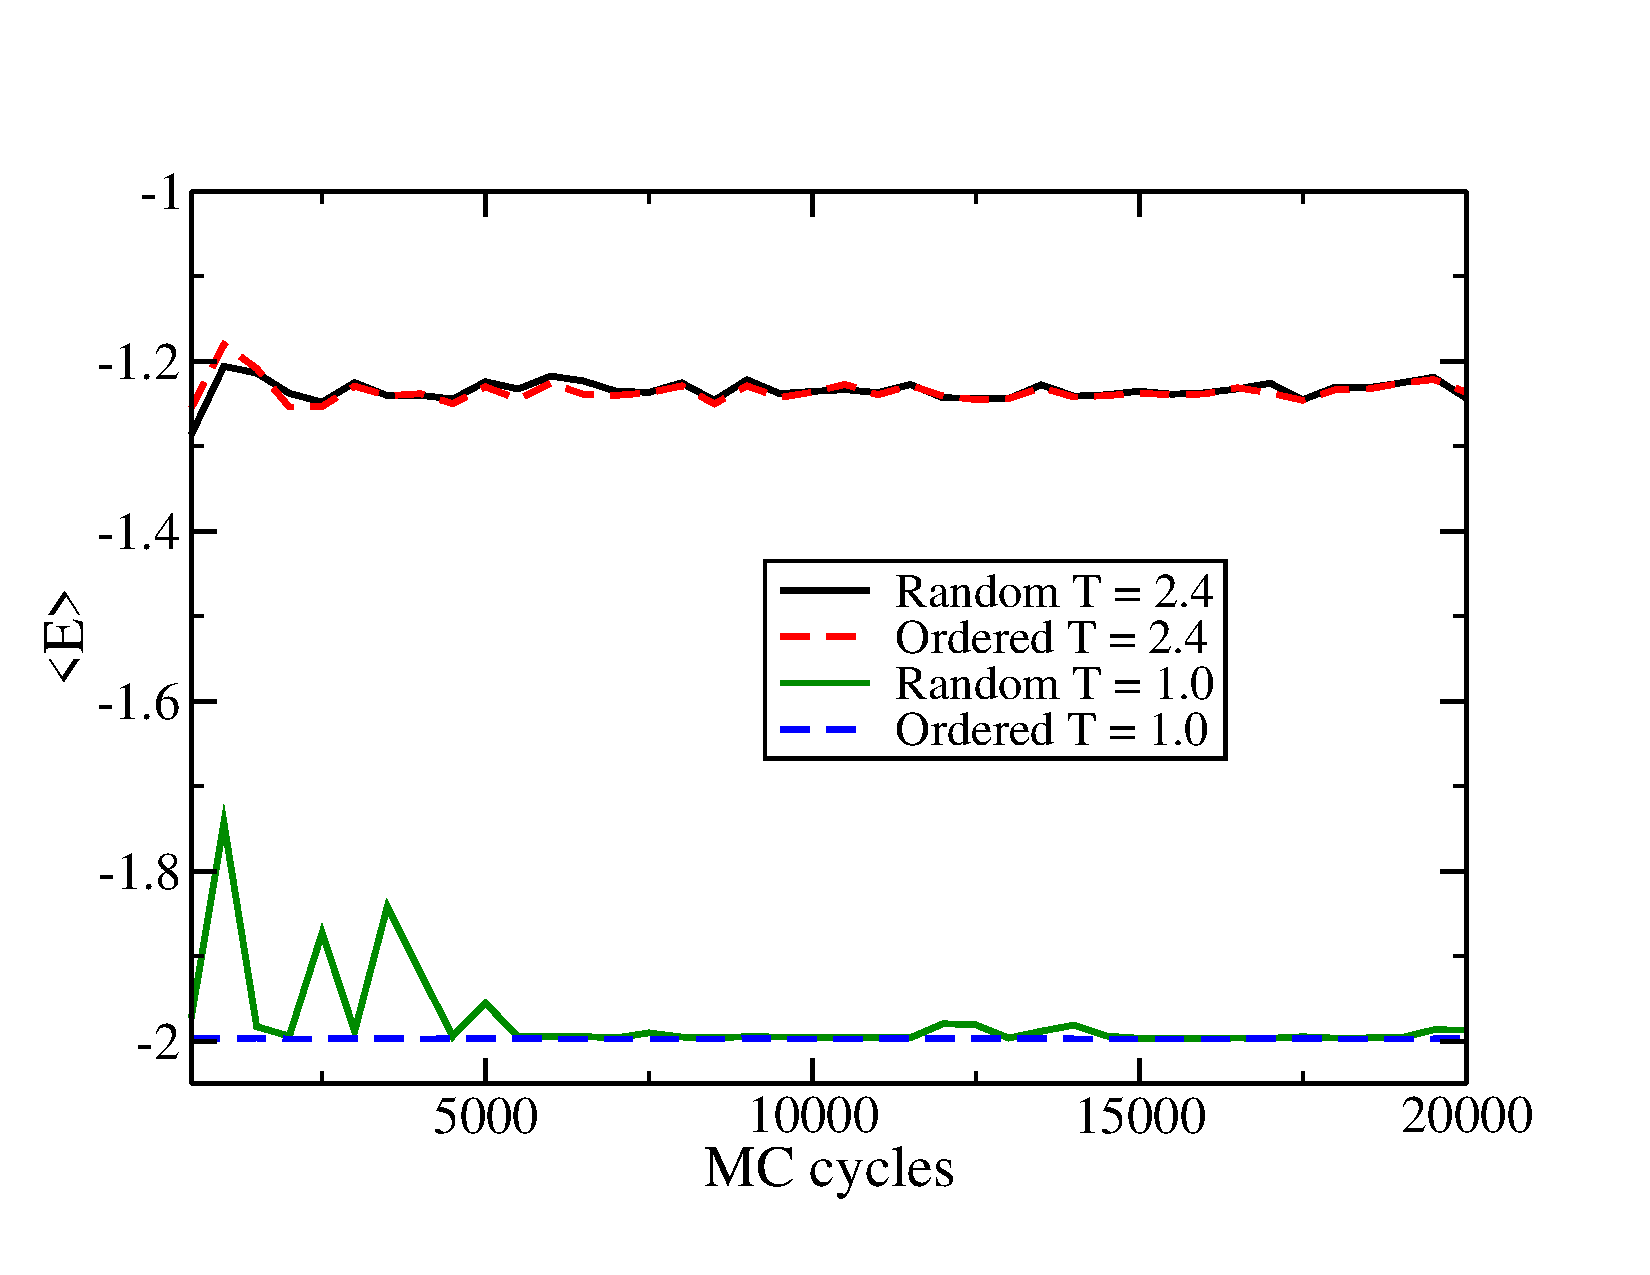
\includegraphics[scale=0.33]{energy_mc.pdf}
\caption{Average energy as a function of the number of Monte Carlo cycles.}
\label{E_mc}
\end{figure}

\begin{figure}[b]
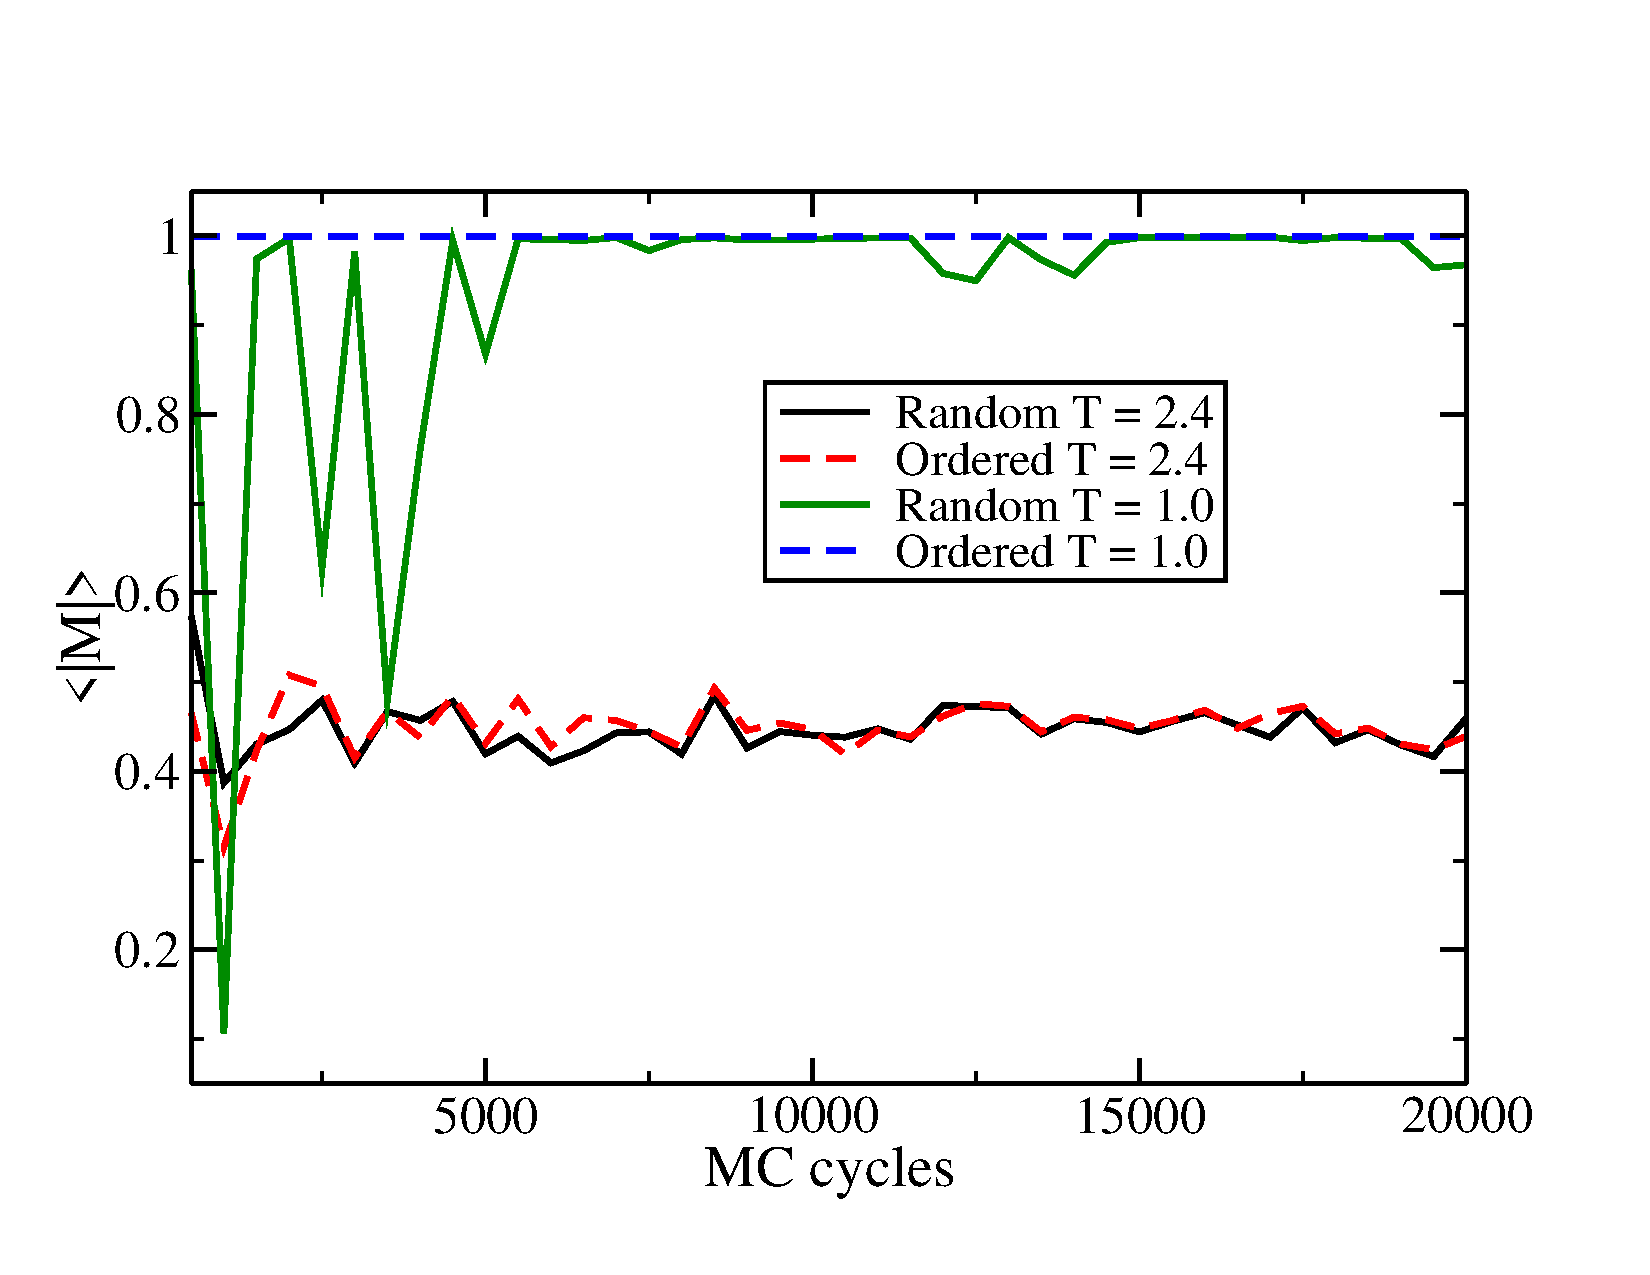
\includegraphics[scale=0.33]{mag_mc.pdf}
\caption{Average magnetization as a function of the number of Monte Carlo cycles.}
\label{M_mc}
\end{figure}

\begin{figure}[t]
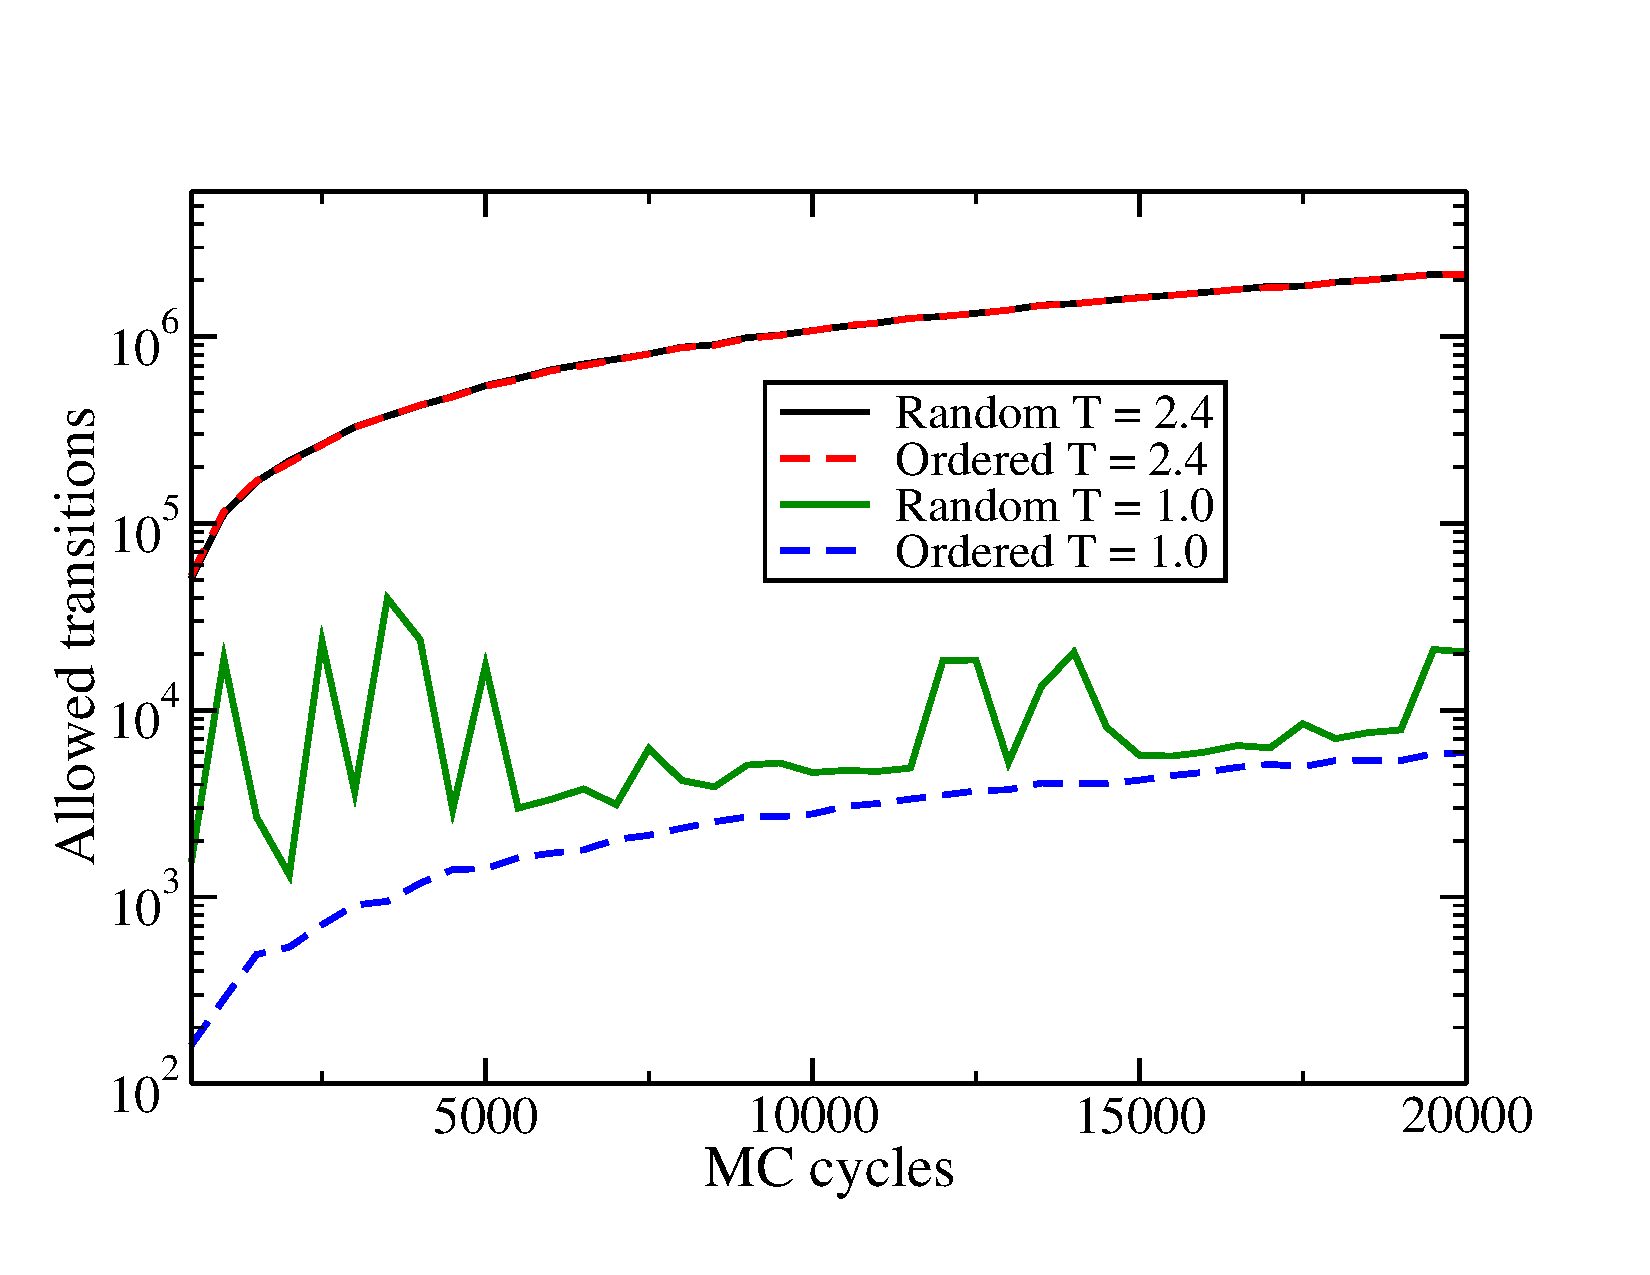
\includegraphics[scale=0.33]{config_mc.pdf}
\caption{Number of allowed transitions as a function of the number of Monte Carlo cycles.}
\label{config_mc}
\end{figure}

Next, we investigate the number of accepted transitions as a function of the number of MC cycles in Figure~\ref{config_mc} and as a fucntion of temperature in Figure~\ref{config_T}. In Figure~\ref{config_mc} we again see that for the higher temperature that the performance is almost independent of the initial configuration, while the random configuration allows more transitions than the ordered configuration for small numbers of MC cycles. In Figure~\ref{config_T} the black solid line corresponds to the initially random configuration and the red dashed curve corresponds to the ordered configuration.

\begin{figure}[b]
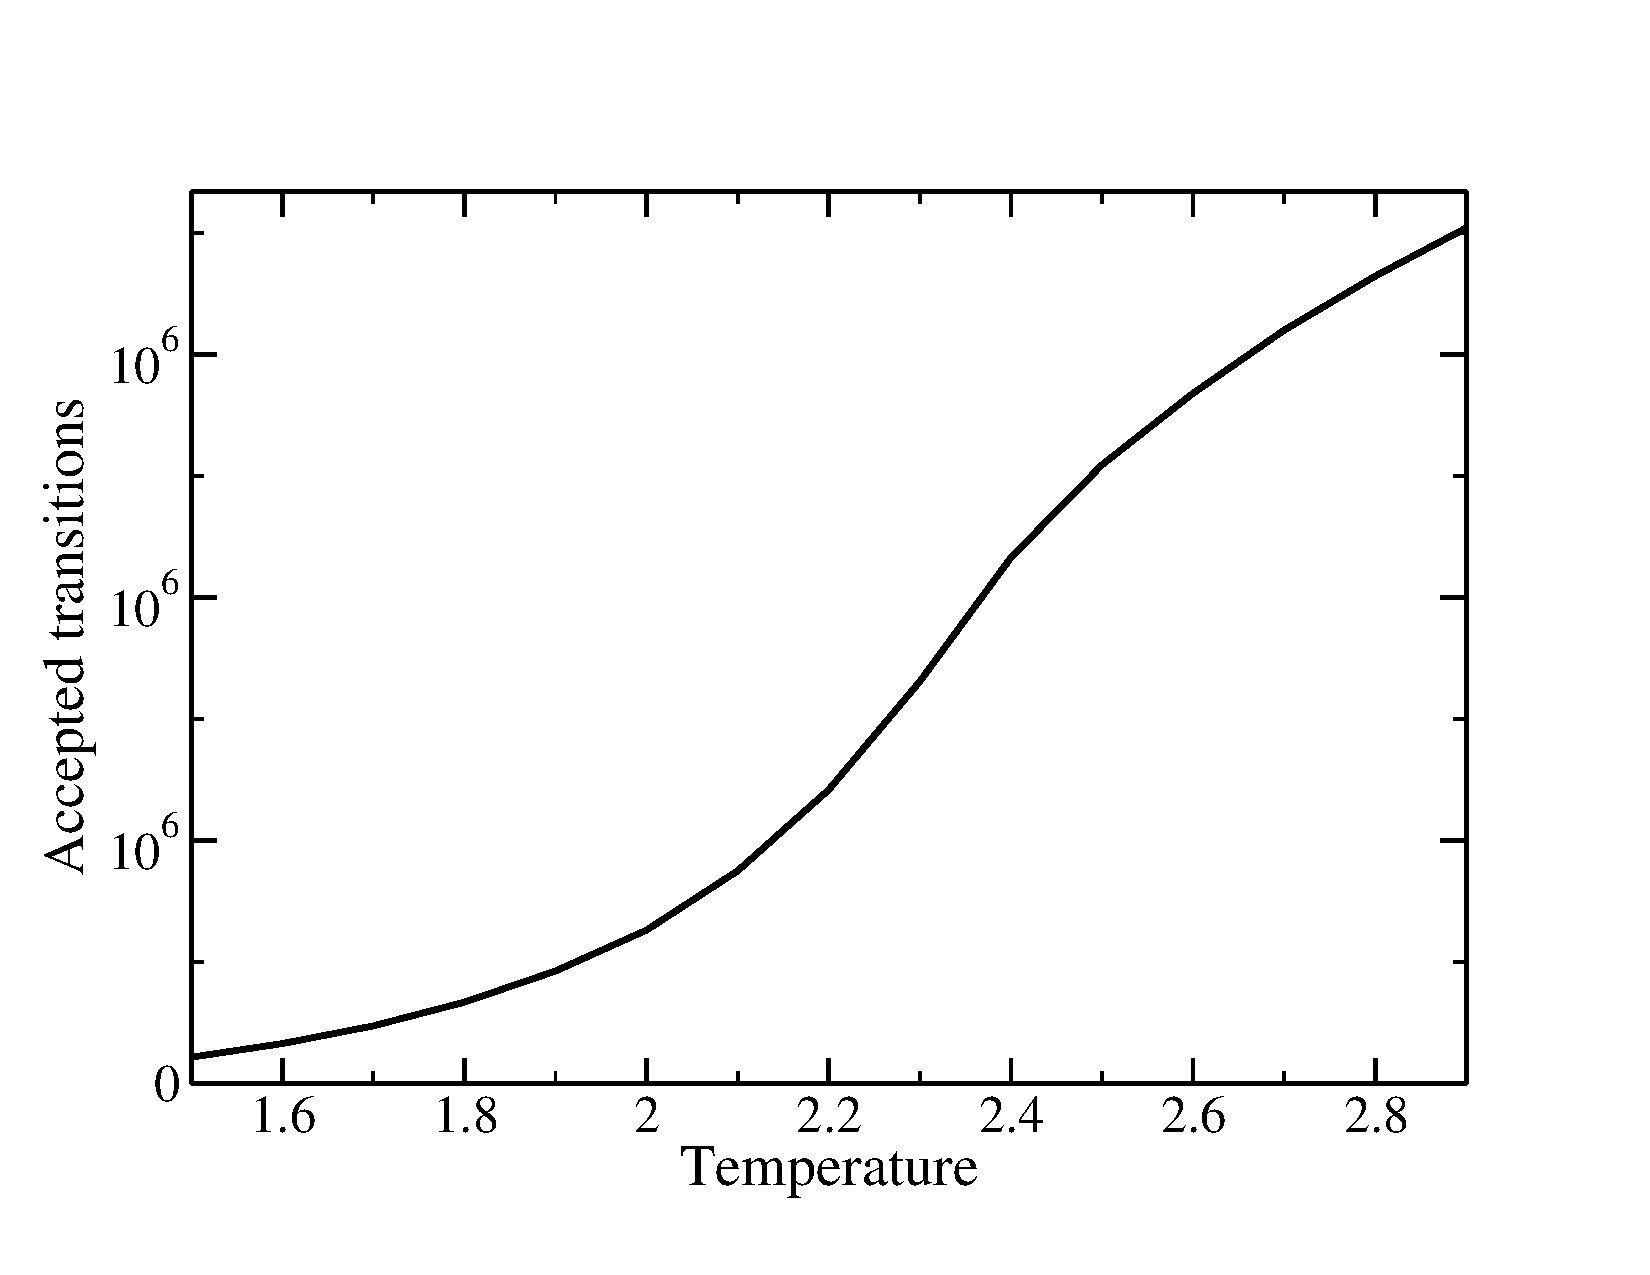
\includegraphics[scale=0.33]{config_T.pdf}
\caption{Number of allowed transitions as a function of temperature for 20000 MC cycles}
\label{config_T}
\end{figure}

\begin{figure}[t]
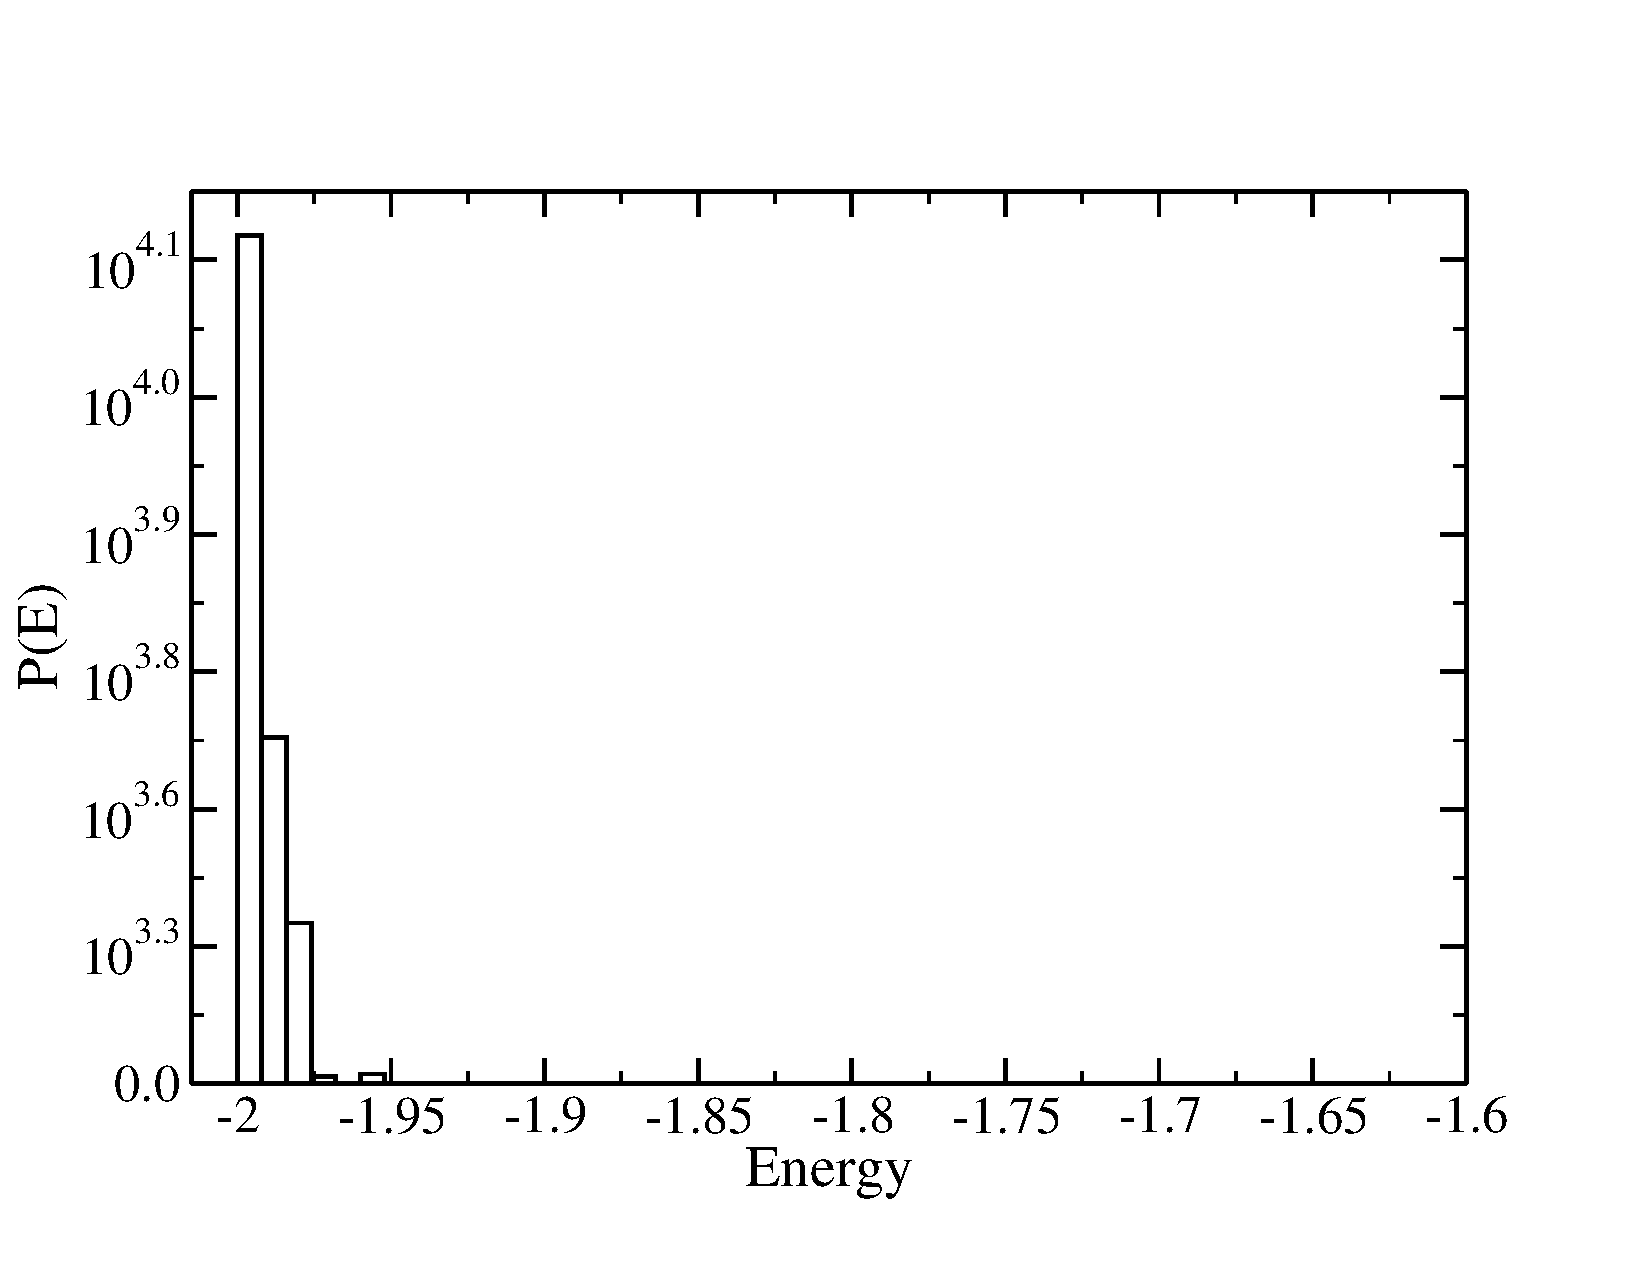
\includegraphics[scale=0.33]{ei_1.pdf}
\caption{Energy probability distribution for 20000 MC cycles at T = 1.0}
\label{ei_1}
\end{figure}

Additionally, we would like to analyze the probability distribution of energies at both high and low temperature. At low temperatures, one expects the distribution to be concentrated around the mean value with small deviations as the configuration starts at the lowest energy state, so the only acccepted energy changes will be those that increase the energy, and a smaller temperature means smaller values will be accepted in the Metropolis algorithm. In contrast, at higher temperatures there should then be a more broad distribution. This is demonstrated by the energy variance, which for T = 2.4 is roughly sixty times larger than for T = 1.0. This is also demonstrated in Figures~\ref{ei_1} and~\ref{ei_2} which show histograms of the accepted energies for T = 1.0 and 2.4 respectively with 20000 MC cycles. In Figure~\ref{ei_1} we see that almost all of the probability is situated in a few bins, while in Figure~\ref{ei_2} the distribution spread over many more energies.

\begin{table}[b]
\centering
\begin{tabular}{|c|c|}
\hline
Temperature & Variance\\
\hline
1.0 & 0.129 \\
2.4 & 7.917 \\
\hline
\end{tabular}
\caption{Energy and magnetization of all possible spin configurations for a 2x2 lattice.}
\label{cycles}
\end{table}

\begin{figure}[t]
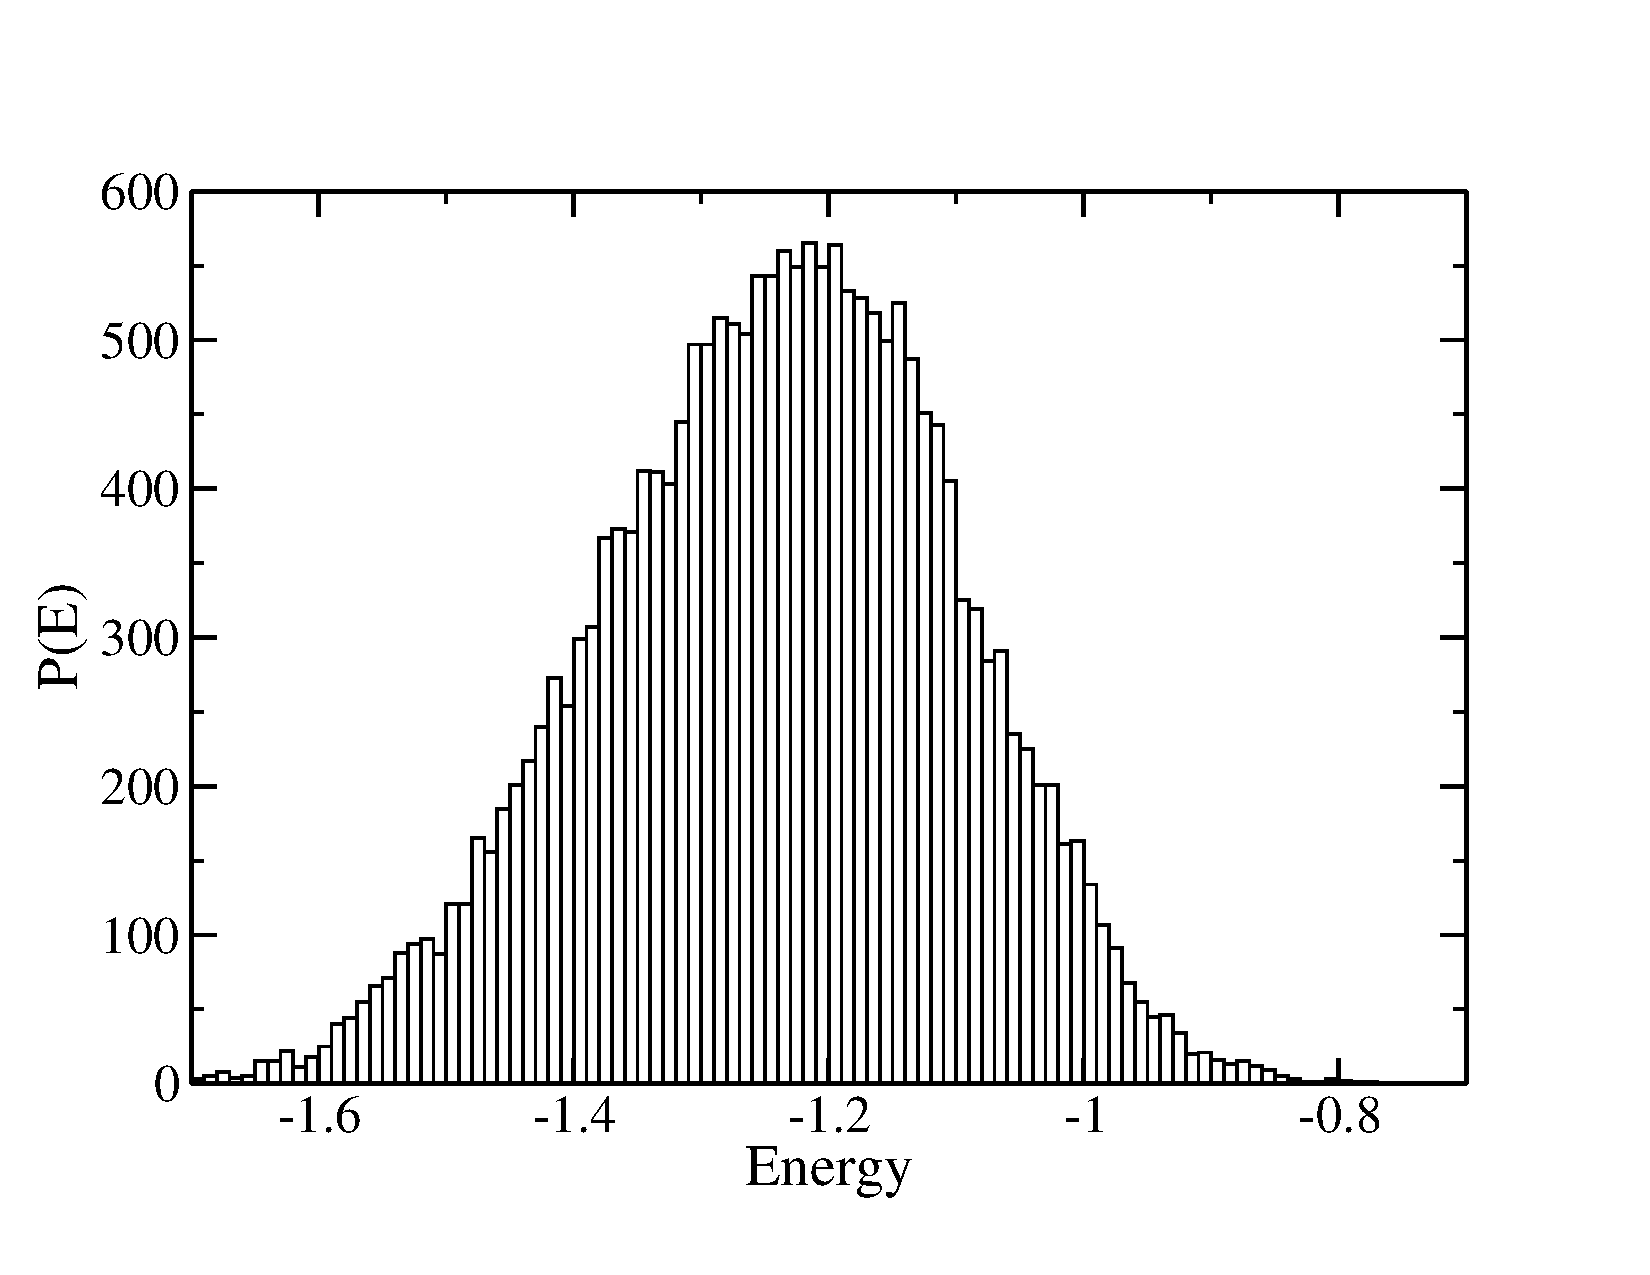
\includegraphics[scale=0.33]{ei_2.pdf}
\caption{Energy probability distribution for 20000 MC cycles at T = 2.4}
\label{ei_2}
\end{figure}

Finally, we ultimately want to investigate the properties of the phase transition, including the critical temperature and the behavior near it. We calculate the average energy, average absolute value of magnetization, heat capacity and magnetic susceptibility in Figures~\ref{ei_2}-\ref{var_m} respectively for lattice sizes of 80x80 (black solid line), 60x60 (red dashed line), 40x40 (green dot dashed line), and 20x20 (blue dotted line). In each we choose a temperature step size of 0.1 and ten thousand MC cycles when outside the range of $T=[2.2,2.4]$ and a temperature step size of 0.02 and one hundred thousand MC cycles inside the range. This is done to save computation time in the areas that are further from the critical temperature and therefore of less interest.

In Figure~\ref{avg_e}, we expect the phase transition to manifest as a discontinuity in the second derivative of the energy, which would manifest as an inflection point. This can be seen for all lattice sizes near $T_C=2.28$. As the head capacity corresponds to the second derivative of the potential, we expect a divergence at the critical point. Since the lattice is finite, this will manifest as a sharp peak, which can also be seen at $T_C=2.26$ in Figure~\ref{var_e}.

Similarly, In Figure~\ref{avg_m} we expect there to be a sharp drop to zero magnetization at the critical temperature. Again due to the finite size of the lattice there will be some deviation from this, but the critical temperature is determined to be $T_C=2.32$. For the susceptibility, the critical temperature is determined to be at $T_C=2.30$.

Using these calculated values and Equations 17-20, the critical temperature for an infinite lattice is computed and compared to the exact result of 2.269~\cite{?} in Table~\ref{comp}. Here we find that the most accurate method of determining the critical temperature was via the average energy, which gave an infinite lattice critical temperature of $T_C=2.268$, which is 0.04\% from the expected value. From the figures, this also appears to be the most stable calculation with lattice size.

\begin{table}[b]
\centering
\begin{tabular}{|c|c|c|c|}
\hline
Method&$T_C$ (N=80) &$T_C$ (N=$\infty$)&Error (\%) \\
\hline
$\langle E\rangle$&2.28&2.268 &0.04\\
$C_V$ &2.26&2.248&0.93\\
$\langle |M|\rangle$&2.32& 2.308&1.72\\
$\chi$&2.30&2.288&0.84\\
\hline
\end{tabular}
\caption{Calculated critical temperatures for a finite lattice and the extrapolated values for an infinite lattice.}
\label{comp}
\end{table}

\begin{figure}[t]
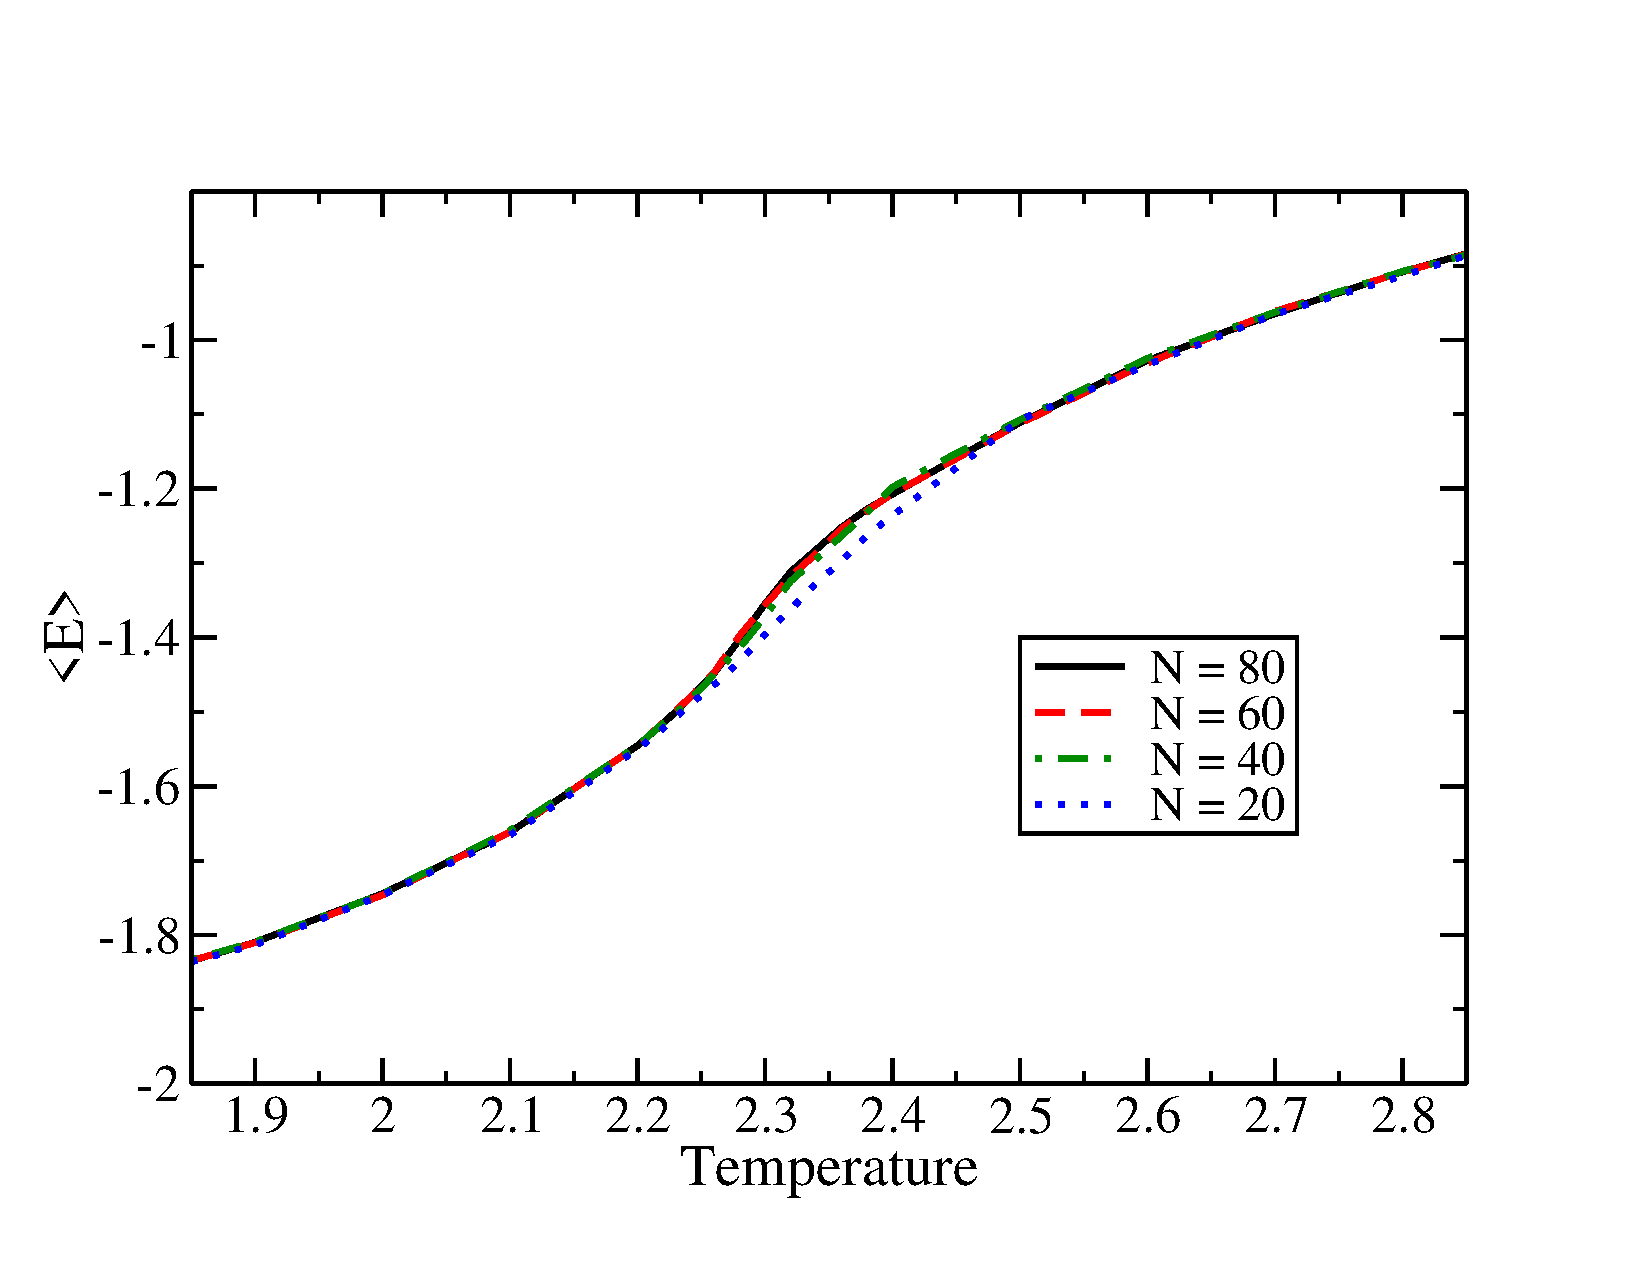
\includegraphics[scale=0.33]{avg_energy.pdf}
\caption{Average energy as a function of temperature for lattice sizes of 20,40,60 and 80.}
\label{avg_e}
\end{figure}


\begin{figure}[b]
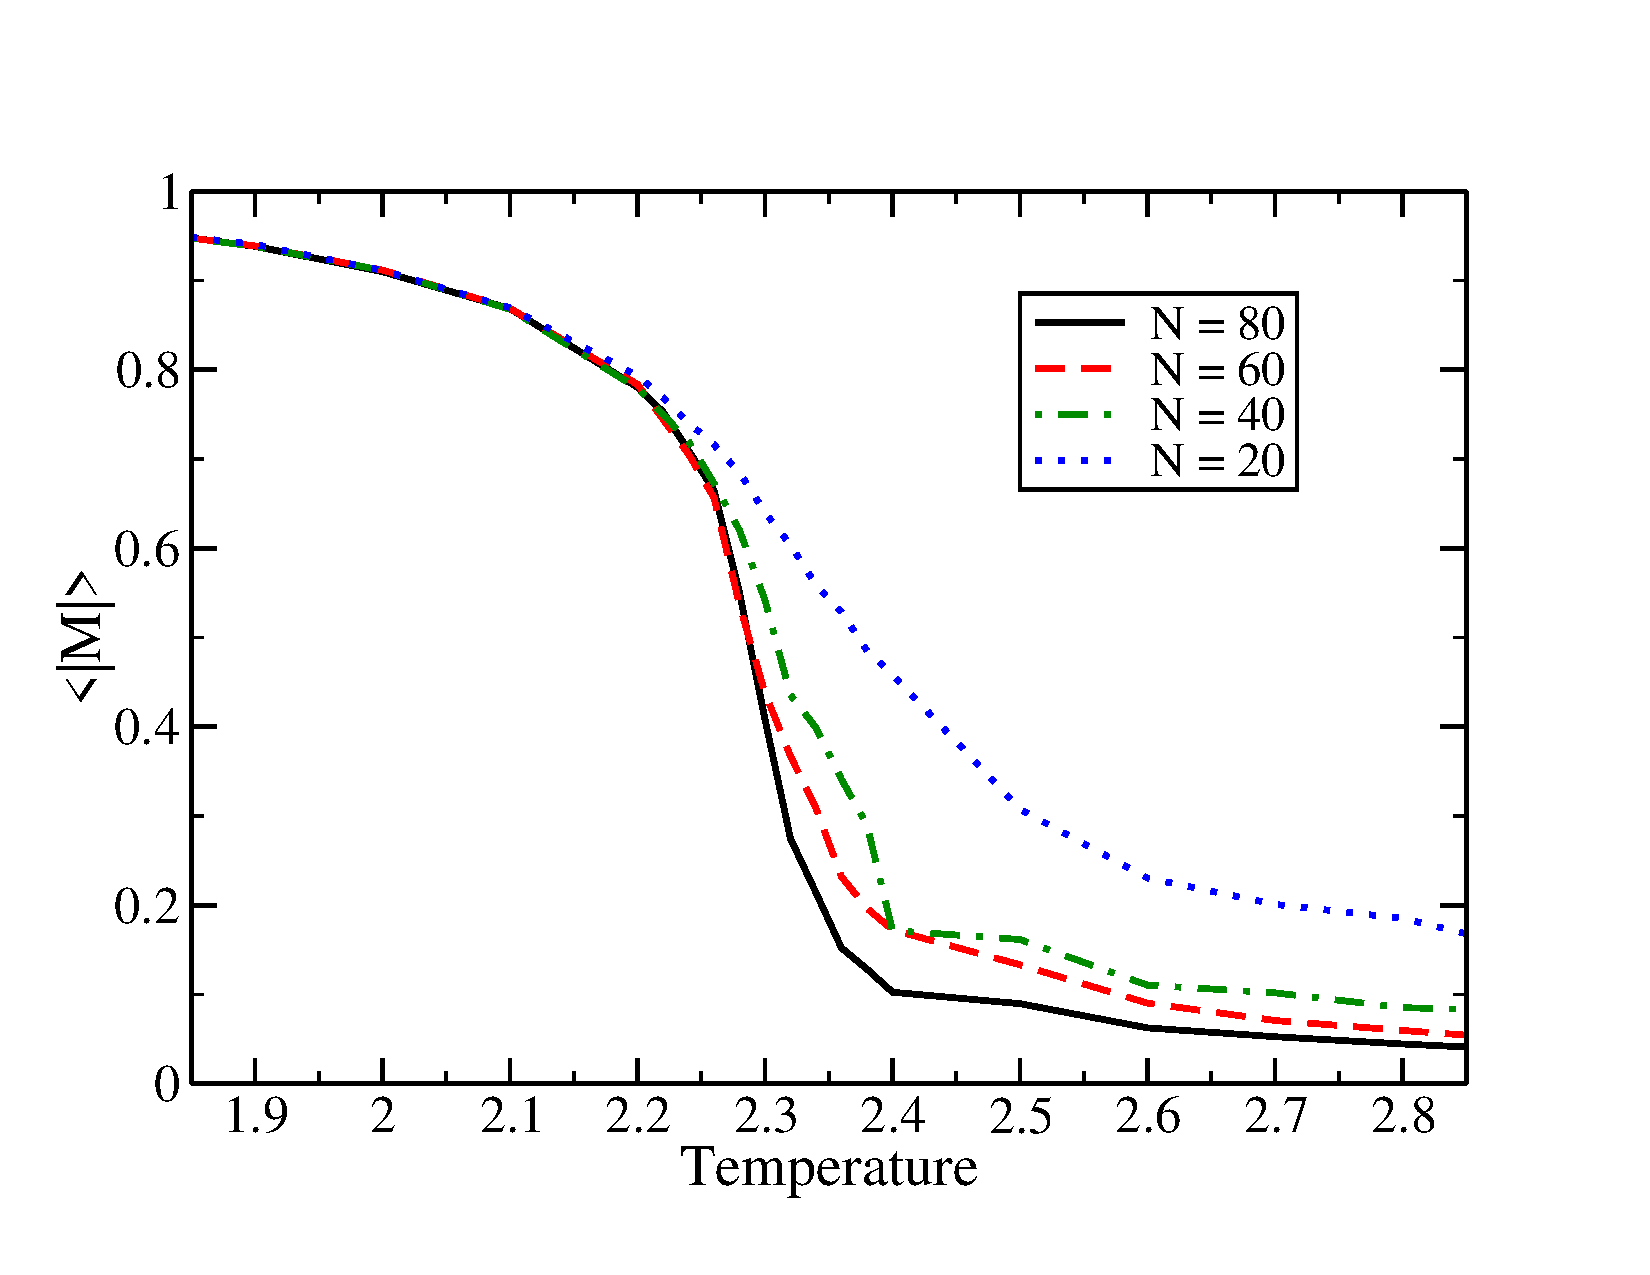
\includegraphics[scale=0.33]{avg_mag.pdf}
\caption{Average absolute value of magnetization as a function of temperature for lattice sizes of 20,40,60 and 80.}
\label{avg_m}
\end{figure}

\begin{figure}[t]
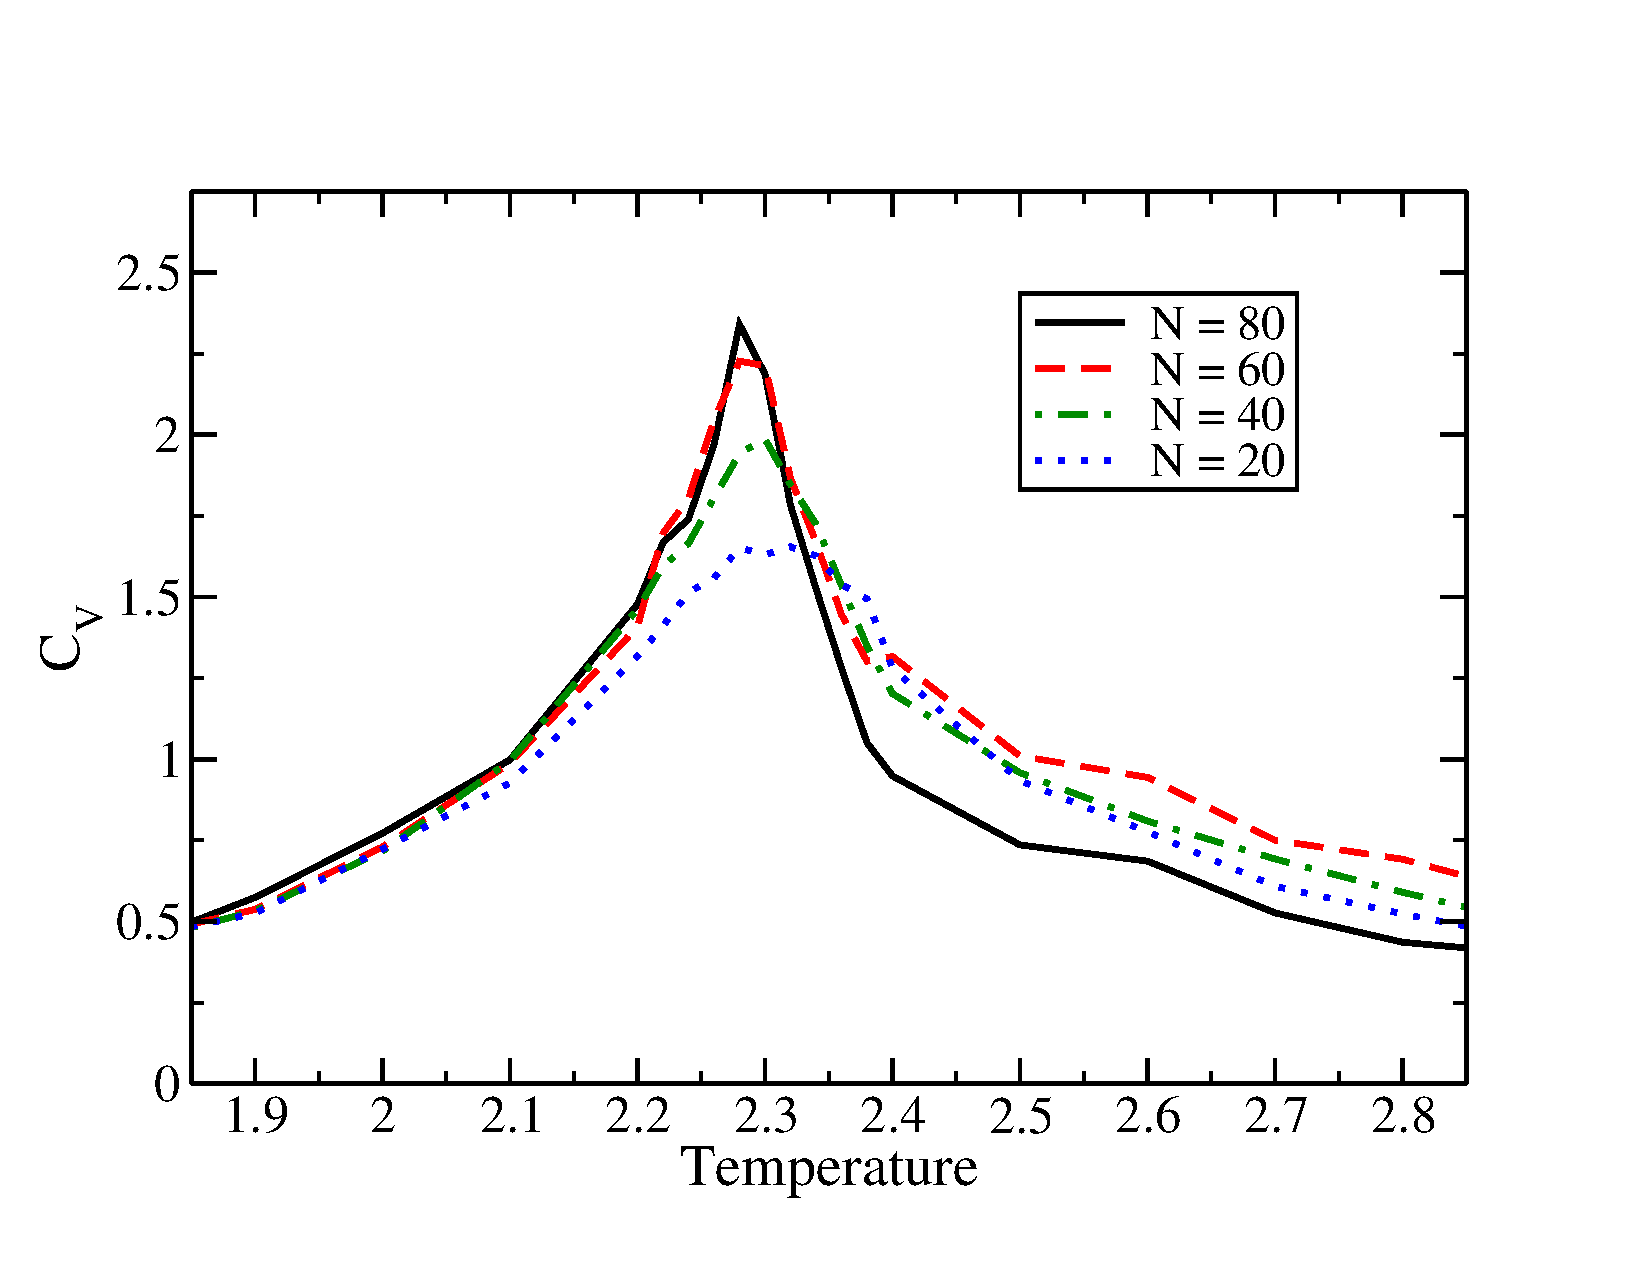
\includegraphics[scale=0.33]{var_energy.pdf}
\caption{Heat capacity as a function of temperature for lattice sizes of 20,40,60 and 80.}
\label{var_e}
\end{figure}

\begin{figure}[b]
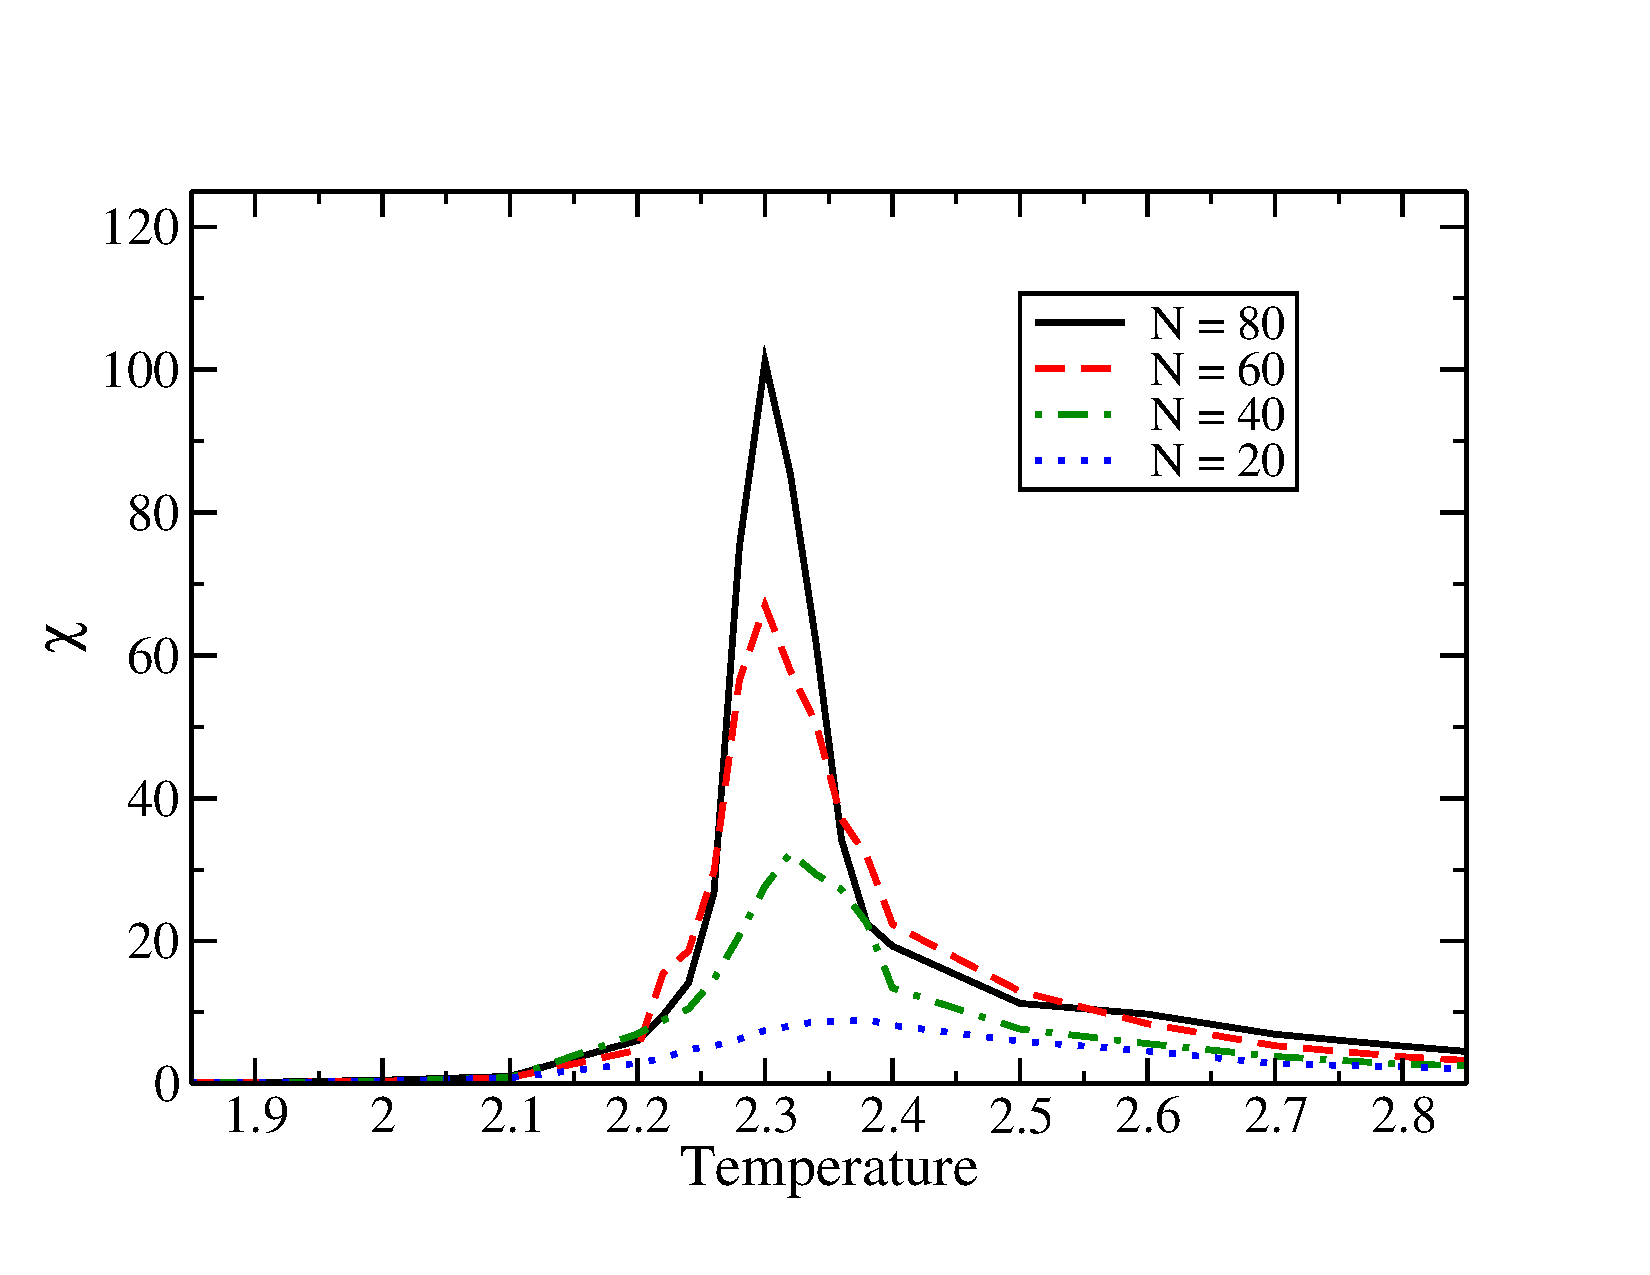
\includegraphics[scale=0.33]{var_mag.pdf}
\caption{Magnetic susceptibility as a function of temperature for lattice sizes of 20,40,60 and 80.}
\label{var_m}
\end{figure}


\section{conclusions}
\label{conc}
In summary, the goal of this work was to simulate phase transitions of magnetic materials via the Ising model. To do this, the stochastic process is simulated by random flipping of spins and the Metropolis algorithm to determine valid transitions. Calculations were performed for the average energy, average square energy, head capacity, average magnetization, average square magnetization and magnetic susceptibility for varying lattice sizes and number of Monte Carlo cycles.

First, we investigated the time to equilibrium for the average energy and magnetization with both a random starting orientation, and an ordered orientation. This was done for both a low and a high temperature. Here it was found that at high temperatures the initial orientation did not effect the number of cycles needed, while it could almost double the number of necessary cycles at low temperatures.

Next, we perform calculations at T = 1.0 and 2.4 and view the energy probability distributions. Here we find that at low temperatures the probability is strongly focussed around one energy with a very small variance. In contrast, at higher energy the Metropolis algorithm has a greater probability of accepting transitions, so the probability distribution is much more broad.

Finally, we plot our observables as a function of temperature in order to extract the critical temperature of the phase transition. As the calculations are performed on a finite lattice the results are transformed using Equations 17-20 and compared to the expected value of 2.269. The best calculation came from the average energy, which gave a critical temperature that was less than 0.1\% different.

%In summary, the goal of this work was to calculate numerically the paths of the planets in the solar system using Newton's law of gravitation. Two methods to calculate the differential equations were used, namely, the Euler method and the velocity Verlet method.

%The Euler method was shown to be unstable in calculating the Earth's orbit in a system which only contained the Earth and sun. In contrast, the Verlet method was stable for practically all step sizes. While the Verlet method was slower, both methods took under one second for a five year simulation, so the difference in timing was negligible. In addition, with the Verlet method we show the importance of the correct initial conditions, as too large of a velocity could cause the system to become unbound.

%Next, we include Jupiter in the model, and explore the dependance of Earth's trajectory on the mass of Jupiter. The calculations are first performed with the physical mass of Jupiter and then with a mass 10 times larger and then 100 times. In all cases the final trajectories were indistinguishable, showing that the sun has the more substantial effect on the orbit of the planets.

There are a number of ways that out code can be improved upon, for example XXX

%There are a number of ways that our code can be improved upon, for example there are more algorithms that could have been explored, such as the Runge-Kutta method~\cite{RK}, which could prove to be more efficient. In addition, the precession of Mercury is known to be incorrect when only newtonian mechanics are considered, so an approximation of the effects of general relativity could be employed to correct for the differences.

% Finally, while the computation time for these examples were small, as moons and other various celestial bodies are added there may be a point in which parallelization of the Verlet algorithm as done in~\cite{omp} with OpenMP and MPI could be helpful. Although, it should be noted that this particular problem includes quite a bit of I/O manipulation, which would require additional effort.

%Overall, we have demonstrated that using Newton's law of gravitation rather than general relativity yields fairly accurate results for the motion of the planets in our solar system. In addition, we have shown that the velocity Verlet algorithm is robust, especially for the chosen application. Finally, these results illustrate the importance of choosing the right tool for the job, as the Euler method failed to produce stable results for even the simplest of cases.



\bibliography{ising}
\end{document}

